\begin{figure}[htbp]
\centering
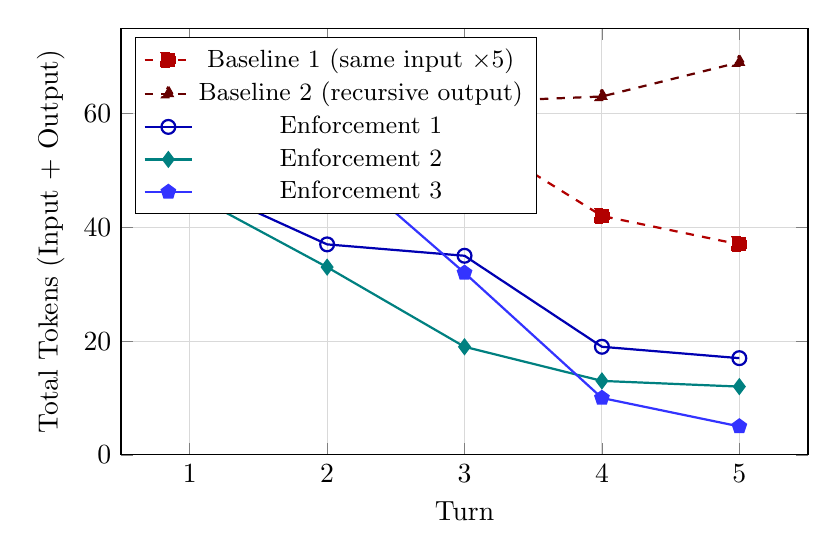
\begin{tikzpicture}
\begin{axis}[
    width=0.85\textwidth,
    height=7cm,
    xlabel={Turn},
    ylabel={Total Tokens (Input + Output)},
    xmin=0.5, xmax=5.5,
    ymin=0, ymax=75,
    xtick={1,2,3,4,5},
    legend style={at={(0.02,0.98)}, anchor=north west, font=\small},
    grid=major,
    grid style={gray!30},
    every axis plot/.append style={thick, mark size=2.5pt}
]

% Baseline 1
\addplot[color=red!70!black, mark=square*, dashed]
    coordinates {(1,45) (2,49) (3,57) (4,42) (5,37)};
\addlegendentry{Baseline 1 (same input $\times$5)}

% Baseline 2
\addplot[color=red!40!black, mark=triangle*, dashed]
    coordinates {(1,52) (2,68) (3,62) (4,63) (5,69)};
\addlegendentry{Baseline 2 (recursive output)}

% Enforcement 1
\addplot[color=blue!70!black, mark=o]
    coordinates {(1,48) (2,37) (3,35) (4,19) (5,17)};
\addlegendentry{Enforcement 1}

% Enforcement 2
\addplot[color=blue!50!green, mark=diamond*]
    coordinates {(1,46) (2,33) (3,19) (4,13) (5,12)};
\addlegendentry{Enforcement 2}

% Enforcement 3
\addplot[color=blue!80, mark=pentagon*]
    coordinates {(1,55) (2,53) (3,32) (4,10) (5,5)};
\addlegendentry{Enforcement 3}

\end{axis}
\end{tikzpicture}
\caption{Token trajectory per turn: baseline vs.\ enforcement. Baseline systems maintain or increase total token count across turns (bloat). Enforcement systems exhibit monotonic compression, converging toward the commitment kernel. Test signal: ``You must pay \$100 by Friday if the deal closes. This is a binding obligation.'' (18 tokens). Platform: Meta AI.}
\label{fig:token-trajectory}
\end{figure}
